\subsection{Prototipo mínimo viable}
Con el fin de desarrollar una aplicacion que permita ejemplificar la tercerizacion de la valoración técnica de profesionales TI usando Estrategias de Gamificación con Énfasis en Ingeniería Web se plantea una serie de tecnologias y arquitectura para llevarla a cabo.

\newline

\textbf{Tecnologías}

\begin{itemize}
    
    \item \textbf{MongoDB Atlas: } MongoDB Atlas es un servicio de Cloud Database (o Base de Datos en la Nube), que te permite crear y administrar tu BBDD Mongo desde cualquier lugar del mundo, a través de su plataforma. 
    
    Además, MongoDB Atlas no solo está orientado a ser accesible desde el navegador, sino que, fue desarrollado con el objetivo de aliviar el trabajo de los desarrolladores, al quitarles la necesidad de instalar y administrar entornos de BBDD, los que a veces pueden ser lentos y engorrosos. Esta va ser la herramienta que vamos a usar para la base de datos.
   
    \vspace{2mm}
        \begin{minipage}{0.9\textwidth}
        \centering
        \captionof{figure}[{Logo MongoDB Atlas}]{ Logo MongoDB Atlas  }
        \label{mongoDB}
         
\includegraphics[width=0.3\textwidth]{Images/mongodb-atlas.png}
          %esto es lo nuevo que agregue
        \fnote{Nota. \textup{Fuente: MongoDB.com}}
    \end{minipage}

    \item \textbf{Node js: }  Node.js, es un entorno en tiempo de ejecución multiplataforma para la capa del servidor (en el lado del servidor) basado en JavaScript. Node.js es un entorno controlado por eventos diseñado para crear aplicaciones escalables, permitiéndote establecer y gestionar múltiples conexiones al mismo tiempo. Gracias a esta característica, no tienes que preocuparte con el bloqueo de procesos, pues no hay bloqueos.
   
    \vspace{2mm}
        \begin{minipage}{0.9\textwidth}
        \centering
        \captionof{figure}[{Logo Node.js}]{ Logo Node.js  }
        \label{nodeJS}
         
\includegraphics[width=0.3\textwidth]{Images/nodejs.png}
          %esto es lo nuevo que agregue
        \fnote{Nota. \textup{Fuente: NODEJS.com}}
    \end{minipage}
    \item \textbf{React js: } React es una biblioteca escrita en JavaScript, desarrollada en Facebook para facilitar la creación de componentes interactivos, reutilizables, para interfaces de usuario. React te ayuda a crear interfaces de usuario interactivas de forma sencilla. Diseña vistas simples para cada estado en tu aplicación, y React se encargará de actualizar y renderizar de manera eficiente los componentes correctos cuando los datos cambien.. Uno de sus puntos más destacados, es que no sólo se utiliza en el lado del cliente, sino que también se puede representar en el servidor, y trabajar juntos.
    
    \vspace{2mm}
        \begin{minipage}{0.9\textwidth}
        \centering
        \captionof{figure}[{Logo React}]{ Logo React  }
        \label{nodeJS}
         
\includegraphics[width=0.2\textwidth]{Images/react.png}
          %esto es lo nuevo que agregue
        \fnote{Nota. \textup{Fuente: react.com}}
    \end{minipage}
    \item \textbf{Vercel: } Vercel ayuda a los equipos de front-end a trabajar de forma más rápida y eficiente combinando las mejores prácticas de desarrollo con un enfoque especializado en el rendimiento del usuario final.Vercel acelera el proceso de creación, prueba e implementación de páginas web al compilar todo el código necesario en un único archivo. A su vez, facilita el seguimiento de los cambios, la depuración de errores y la garantía de un estilo coherente en todas las páginas. Esta va ser nuestra herramienta para hacer el despligue de nuestro front-end.

    \vspace{2mm}
        \begin{minipage}{0.9\textwidth}
        \centering
        \captionof{figure}[{Logo Vercel}]{ Logo Vercel  }
        \label{vercel}
         
\includegraphics[width=0.2\textwidth]{Images/vercel-logo-freelogovectors.net.jpg}
          %esto es lo nuevo que agregue
        \fnote{Nota. \textup{Fuente: vercel.com}}
    \end{minipage}
    
    \item \textbf{Heroku: } Heroku es una plataforma como servicio (PaaS) de computación en la Nube que soporta distintos lenguajes de programación.La red Heroku ejecuta las aplicaciones del cliente en contenedores virtuales que se ejecutan en un entorno de tiempo real, heroku llama a esto contenedores, Dynos. Estos Dynos pueden ejecutar código escrito en Node, Ruby, PHP, Go, Scala, Python, Java o Clojure. Heroku también proporciona buildpacks personalizados con los que el desarrollador puede implementar aplicaciones en cualquier otro lenguaje. Heroku le permite al desarrollador escalar la aplicación instantáneamente tan solo incrementando el número de dyno o ejecutando la aplicación en un dyno más potente. Esta va ser nuestra herramienta para hacer el despliegue de nuestro back-end.

    \vspace{2mm}
        \begin{minipage}{0.9\textwidth}
        \centering
        \captionof{figure}[{Logo Heroku}]{ Logo Heroku  }
        \label{heroku}
         
\includegraphics[width=0.3\textwidth]{Images/Heroku_logo.svg.png}
        \fnote{Nota. \textup{Fuente: herokuio.com}}
    \end{minipage}
\end{itemize}

%\begin{adjustwidth}{35pt}{}
%\end{adjustwidth}
\vspace{5mm}
\textbf{Arquitectura} 
\begin{itemize}
    
    \item \textbf{Arquitectura de micro servicios: } La arquitectura de micro-servicios es un método de desarrollo de aplicaciones software que funciona como un conjunto de pequeños servicios que se ejecutan de manera independiente y autónoma, proporcionando una funcionalidad de negocio completa. En ella, cada micro-servicio es un código que puede estar en un lenguaje de programación diferente, y que desempeña una función específica. Los micro servicios se comunican entre sí a través de APIs, y cuentan con sistemas de almacenamiento propios, lo que evita la sobrecarga y caída de la aplicación.
    
    Esta es la arquitectura elegida para la parte del back-end, por medio de esta es posible implementar cada servicio que requiere nuestro negocio que posteriormente sera desplegado en Heroku.
    
     \vspace{2mm}
     \begin{minipage}{0.9\textwidth}
        \centering
        \captionof{figure}[{Arquitectura de Micro servicios.}]{ Ejemplo Arquitectura de microservicios. }
        \label{microservicios}
         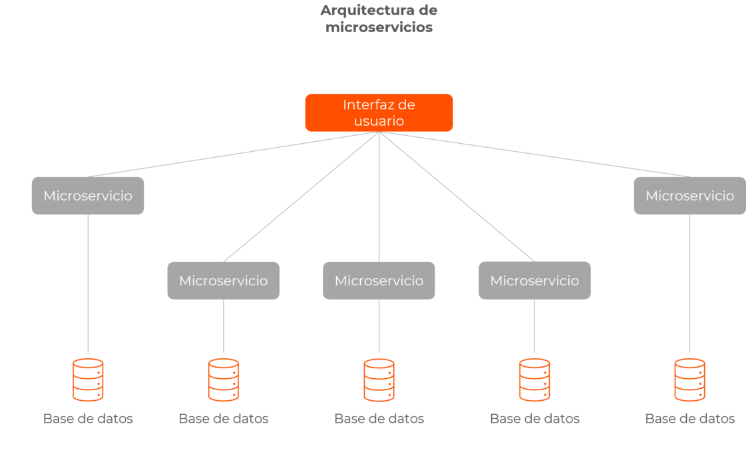
\includegraphics[width=0.9\textwidth]{Images/microservicios.png}
        \fnote{Nota. \textup{Fuente: decidesoluciones.es/arquitectura-de-microservicios}}
    \end{minipage}
    
    \item \textbf{Arquitectura hexagonal: }Uno de los patrones de diseño de arquitectura de software más utilizados es el de la Arquitectura Hexagonal (Hexagonal Architecture), también conocida como arquitectura de Puertos y Adaptadores (Ports and Adapters), dada a conocer por Alistair Cockburn.

    La finalidad principal de este patrón es dividir nuestra aplicación en distintas capas, permitiendo su evolución de manera aislada y responsabilizando a cada entidad de una funcionalidad única.La idea de representar esta arquitectura con un hexágono es debido a la facilidad que presenta el asociar el concepto teórico con el concepto visual, puesto que dentro de dicho hexágono es donde se encuentra nuestro código base, llamado dominio, y cada uno de sus laterales es una interacción hacia un servicio externo

    \vspace{2mm}
     \begin{minipage}{0.9\textwidth}
        \centering
        \captionof{figure}[{Arquitectura Hexagonal.}]{ Ejemplo Arquitectura Hexagonal. }
        \label{hexagonal}
         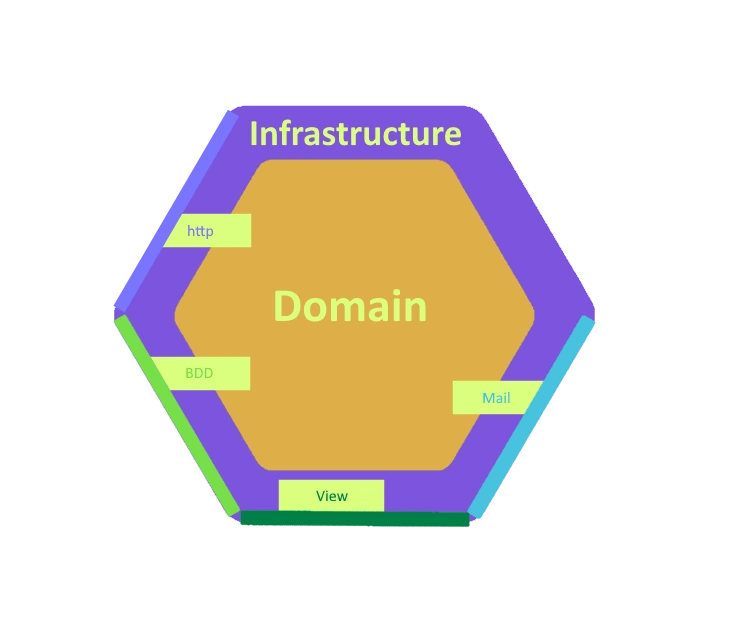
\includegraphics[width=0.7\textwidth]{Images/hexagonal.png}
        \fnote{Nota. \textup{Fuente: https://softwarecrafters.io/react/arquitectura-hexagonal-frontend}}
    \end{minipage}
    
\end{itemize}

\textbf{Infraestructura }
\newline
La computación en la nube es un modelo de entrega donde el almacenamiento, los servidores, las aplicaciones y otros elementos se entregan por Internet. Se entrega bajo demanda como servicio, en general como pago por consumo. «La nube» no es un lugar físico, sino un método de gestión de recursos de TI que sustituye principalmente las máquinas locales y los centros de datos privados. En el modelo de computación en la nube, los usuarios acceden a los recursos virtuales de computación, red y almacenamiento que están disponibles en línea a través de un proveedor remoto. En lugar de tener que comprar y mantener una computación extensiva, almacenamiento y otra infraestructura de TI, como también tener experiencia interna disponible para la gestión de estos equipos, gran parte de esta responsabilidad, en cambio, le corresponde al proveedor de servicios de nube. \cite{glosario_2022}.
\newline
\textbf{Software as a Service (SaaS) :}
Para este proyecto se va trabajar con el servicio SaaS que ofrece la computación en la nube ya que se adapta mejor al desarrollo que se va implementar.dado que es el mas cómodo debido a que se evitan procesos de mantenimiento, actualizaciones y gestión de licencias, a partir que el software se encuentra alojado de manera 100 \%& virtual y los usuarios solo necesitan acceder a ellos desde cualquier lugar. En términos generales, la conversación sobre SaaS se trata de aplicaciones de usuario final. \cite{microsoftazure_2022}


\textbf{Requerimientos}

\begin{enumerate}
    \item Funcionales
        
        
        
        \vspace{2mm}
        \begin{minipage}{0.8\textwidth}
        \centering
        \captionof{table}[{Requerimiento funcional RF-001.}]{ Requerimiento funcional RF-001. }
        \label{req1}
         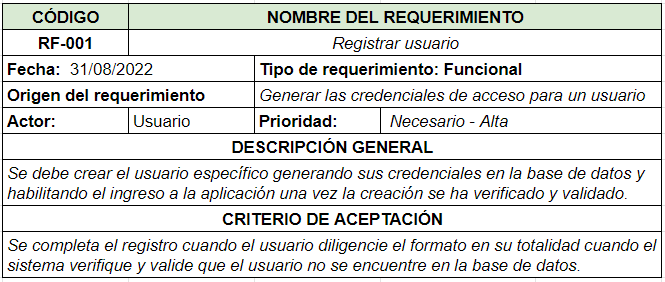
\includegraphics[width=1\textwidth]{Images/1.png}
        \fnote{Nota. \textup{Fuente : Autores.}}
        \end{minipage}
        
        \vspace{2mm}
        \begin{minipage}{0.9\textwidth}
        \centering
        \captionof{table}[{Requerimiento funcional RF-002.}]{ Requerimiento funcional RF-002. }
        \label{req2}
         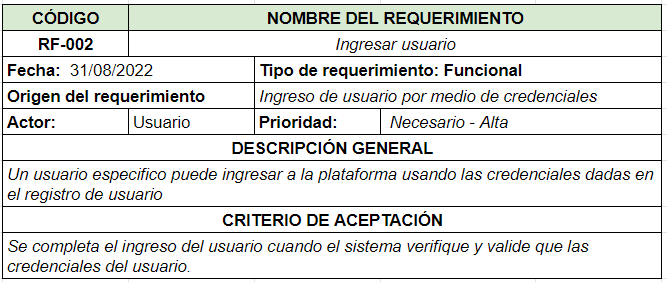
\includegraphics[width=1\textwidth]{Images/2.png}
        \fnote{Nota. \textup{Fuente : Autores.}}
        \end{minipage}
        
        \vspace{2mm}
        \begin{minipage}{0.9\textwidth}
        \centering
        \captionof{table}[{Requerimiento funcional RF-003.}]{ Requerimiento funcional RF-003. }
        \label{req3}
         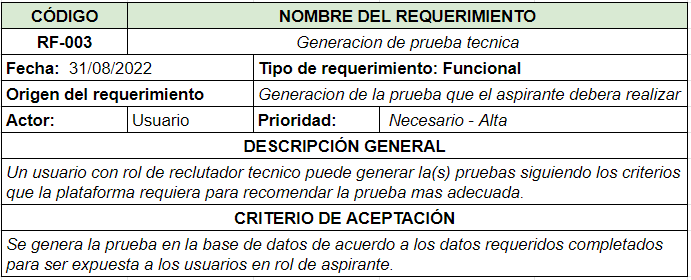
\includegraphics[width=1\textwidth]{Images/3.png}
        \fnote{Nota. \textup{Fuente : Autores.}}
        \end{minipage}
        
        \vspace{2mm}
        \begin{minipage}{0.9\textwidth}
        \centering
        \captionof{table}[{Requerimiento funcional RF-004.}]{ Requerimiento funcional RF-004. }
        \label{req4}
         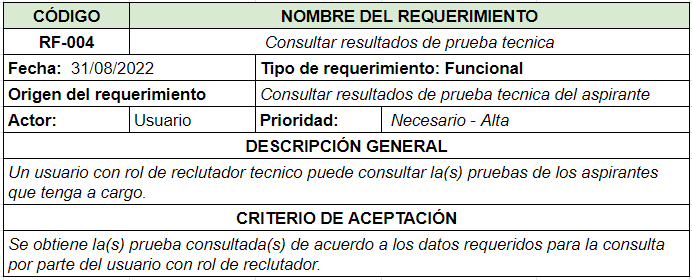
\includegraphics[width=1\textwidth]{Images/4.png}
        \fnote{Nota. \textup{Fuente : Autores.}}
        \end{minipage}
        
        \vspace{2mm}
        \begin{minipage}{0.9\textwidth}
        \centering
        \captionof{table}[{Requerimiento funcional RF-005.}]{ Requerimiento funcional RF-005. }
        \label{req5}
         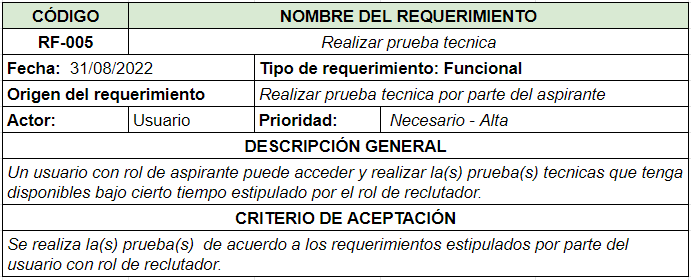
\includegraphics[width=1\textwidth]{Images/5.png}
        \fnote{Nota. \textup{Fuente : Autores.}}
        \end{minipage}
        
        \vspace{2mm}
        \begin{minipage}{0.9\textwidth}
        \centering
        \captionof{table}[{Requerimiento funcional RF-006.}]{ Requerimiento funcional RF-006. }
        \label{req6}
         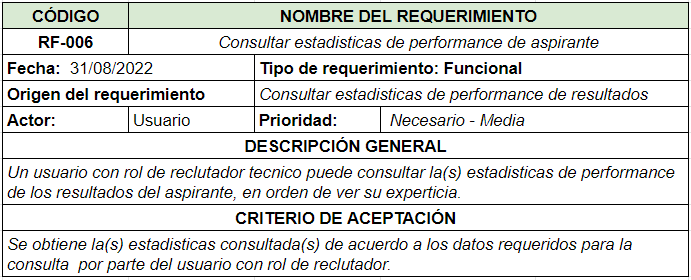
\includegraphics[width=1\textwidth]{Images/6.png}
        \fnote{Nota. \textup{Fuente : Autores.}}
        \end{minipage}
        
        \vspace{2mm}
        \begin{minipage}{0.9\textwidth}
        \centering
        \captionof{table}[{Requerimiento funcional RF-007.}]{ Requerimiento funcional RF-007. }
        \label{req7}
         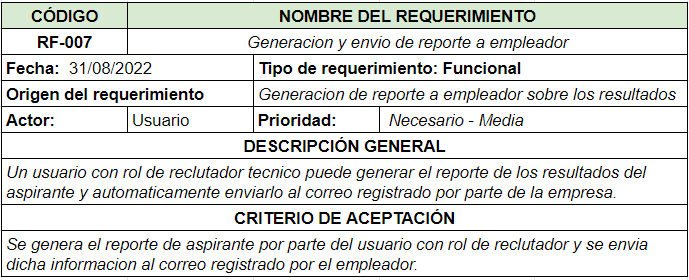
\includegraphics[width=1\textwidth]{Images/7.png}
        \fnote{Nota. \textup{Fuente : Autores.}}
        \end{minipage}
        
        \vspace{2mm}
        \begin{minipage}{0.9\textwidth}
        \centering
        \captionof{table}[{Requerimiento funcional RF-008.}]{ Requerimiento funcional RF-008. }
        \label{req8}
         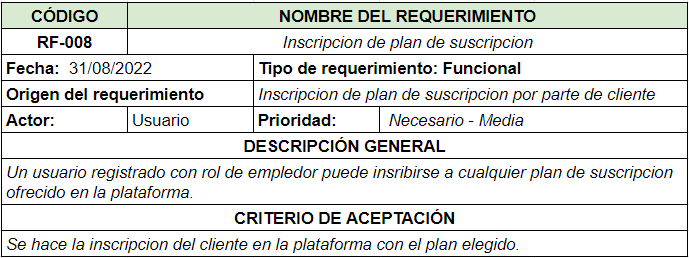
\includegraphics[width=1\textwidth]{Images/8.png}
        \fnote{Nota. \textup{Fuente : Autores.}}
        \end{minipage}
        
    \item No funcionales
    
        
        \vspace{2mm}
        \begin{minipage}{0.9\textwidth}
        \centering
        \captionof{table}[{Requerimiento no funcional RNF-001.}]{ Requerimiento no funcional RNF-001. }
        \label{reqnf1}
         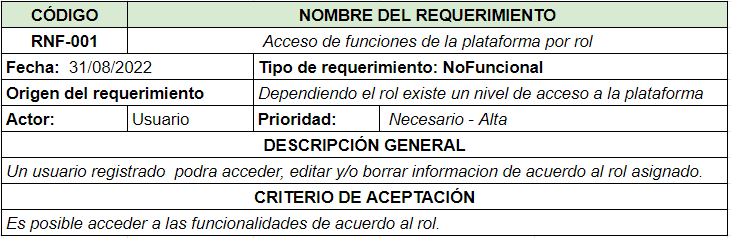
\includegraphics[width=1\textwidth]{Images/nf1.png}
        \fnote{Nota. \textup{Fuente : Autores.}}
        \end{minipage}
        
        \vspace{2mm}
        \begin{minipage}{0.9\textwidth}
        \centering
        \captionof{table}[{Requerimiento no funcional RNF-002.}]{ Requerimiento no funcional RNF-002. }
        \label{reqnf2}
         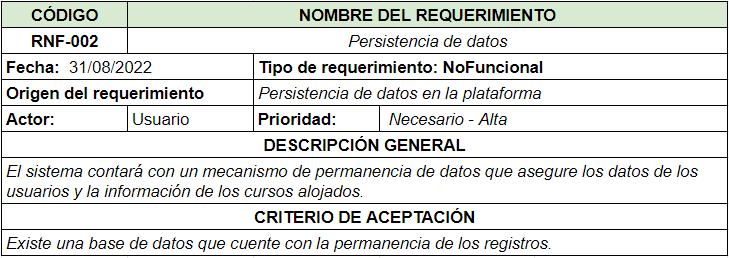
\includegraphics[width=1\textwidth]{Images/nf2.png}
        \fnote{Nota. \textup{Fuente : Autores.}}
        \end{minipage}

        \vspace{2mm}
        \begin{minipage}{0.9\textwidth}
        \centering
        \captionof{table}[{Requerimiento no funcional RNF-003.}]{ Requerimiento no funcional RNF-003. }
        \label{reqnf3}
         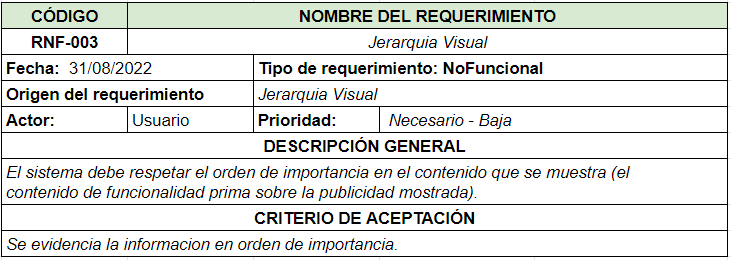
\includegraphics[width=1\textwidth]{Images/nf3.png}
        \fnote{Nota. \textup{Fuente : Autores.}}
        \end{minipage}
        
\end{enumerate}
\newline
\textbf{Casos de uso}
    
    \vspace{2mm}
    \begin{minipage}{0.9\textwidth}
    \centering
    \captionof{figure}[{Caso de uso RF-001.}]{ Caso de uso RF-001. }
    \label{caso1}
     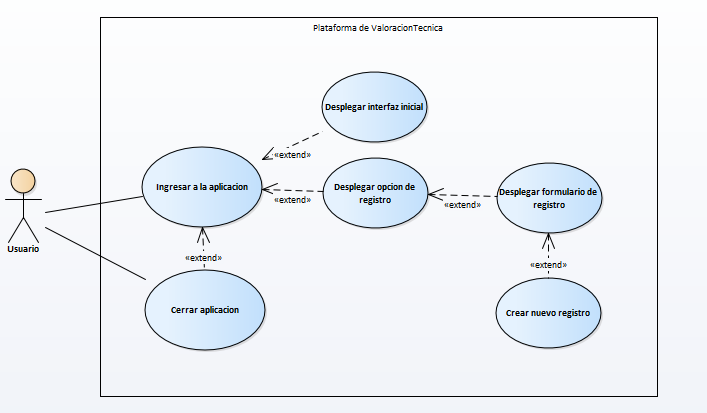
\includegraphics[width=0.9\textwidth]{Images/casoUso1.png}
    \fnote{Nota. \textup{Fuente : Autores.}}
    \end{minipage}
    
    \vspace{2mm}
    \begin{minipage}{0.9\textwidth}
    \centering
    \captionof{figure}[{Caso de uso RF-002.}]{ Caso de uso RF-002. }
    \label{caso2}
     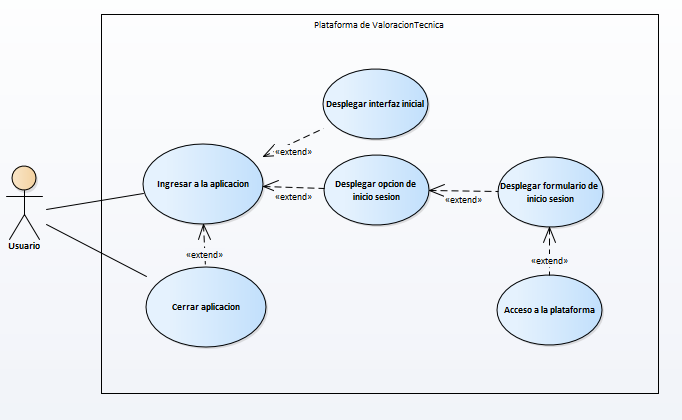
\includegraphics[width=0.9\textwidth]{Images/casoUso2.png}
    \fnote{Nota. \textup{Fuente : Autores.}}
    \end{minipage}
    
    \vspace{2mm}
    \begin{minipage}{0.9\textwidth}
    \centering
    \captionof{figure}[{Caso de uso RF-003.}]{ Caso de uso RF-003. }
    \label{caso3}
     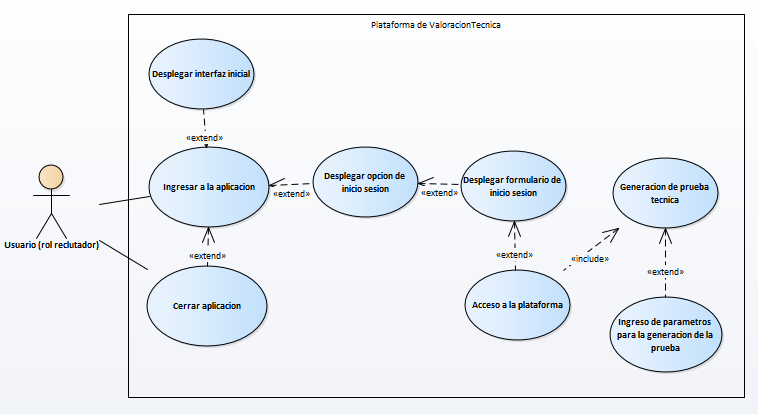
\includegraphics[width=0.9\textwidth]{Images/casoUso3.png}
    \fnote{Nota. \textup{Fuente : Autores.}}
    \end{minipage}
    
    \vspace{2mm}
    \begin{minipage}{0.9\textwidth}
    \centering
    \captionof{figure}[{Caso de uso RF-004.}]{ Caso de uso RF-004. }
    \label{caso4}
     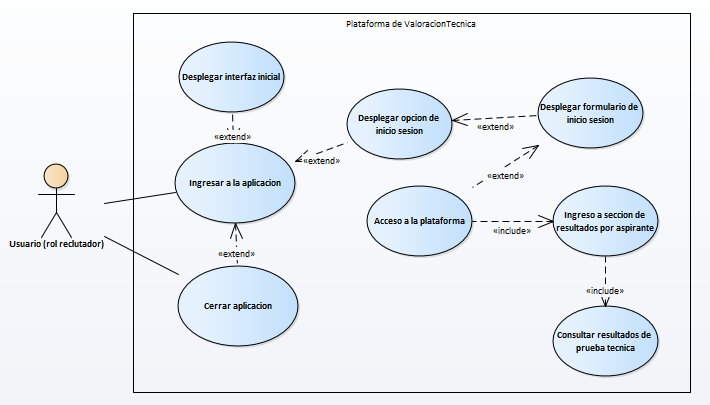
\includegraphics[width=0.9\textwidth]{Images/casoUso4.png}
    \fnote{Nota. \textup{Fuente : Autores.}}
    \end{minipage}
    
    \vspace{2mm}
    \begin{minipage}{0.9\textwidth}
    \centering
    \captionof{figure}[{Caso de uso RF-005.}]{ Caso de uso RF-005. }
    \label{caso1}
     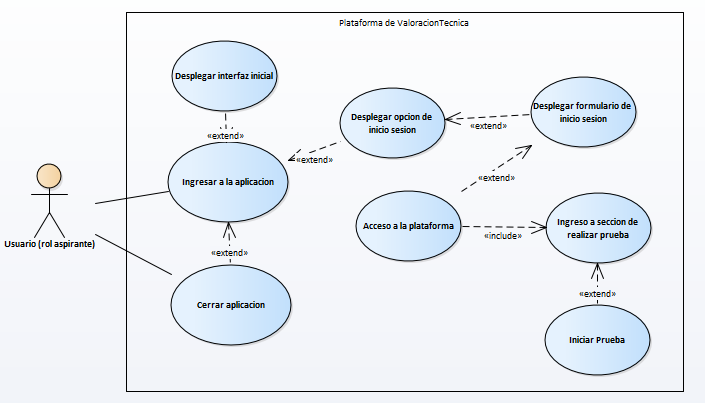
\includegraphics[width=0.9\textwidth]{Images/casoUso5.png}
    \fnote{Nota. \textup{Fuente : Autores.}}
    \end{minipage}
    
    \vspace{2mm}
    \begin{minipage}{0.9\textwidth}
    \centering
    \captionof{figure}[{Caso de uso RF-006.}]{ Caso de uso RF-006. }
    \label{caso1}
     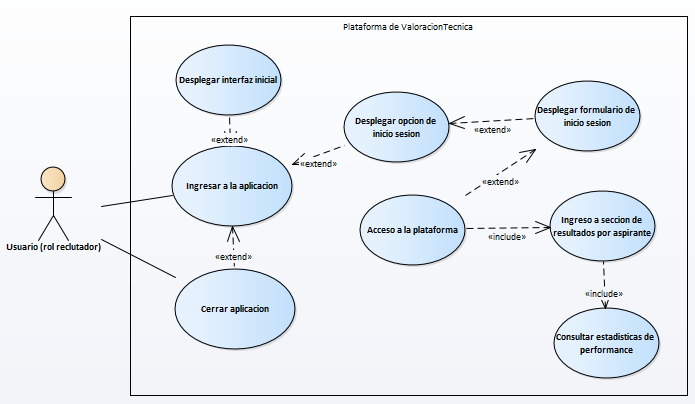
\includegraphics[width=0.9\textwidth]{Images/casoUso6.png}
    \fnote{Nota. \textup{Fuente : Autores.}}
    \end{minipage}
    
    \vspace{2mm}
    \begin{minipage}{0.9\textwidth}
    \centering
    \captionof{figure}[{Caso de uso RF-007.}]{ Caso de uso RF-007. }
    \label{caso1}
     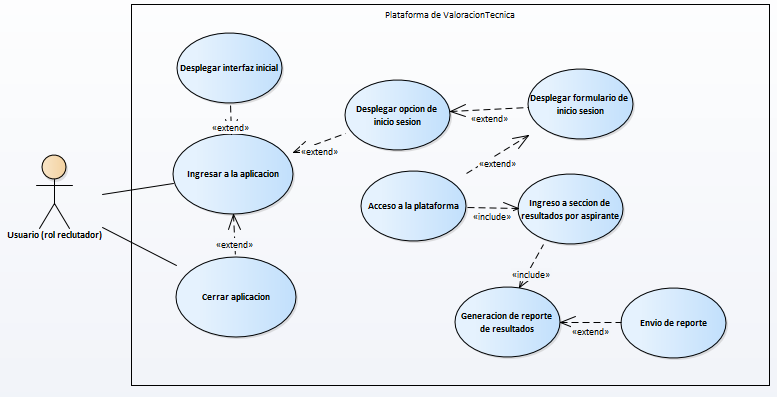
\includegraphics[width=0.9\textwidth]{Images/casoUso7.png}
    \fnote{Nota. \textup{Fuente : Autores.}}
    \end{minipage}
    
    \vspace{2mm}
    \begin{minipage}{0.9\textwidth}
    \centering
    \captionof{figure}[{Caso de uso RF-008.}]{ Caso de uso RF-008. }
    \label{caso8}
     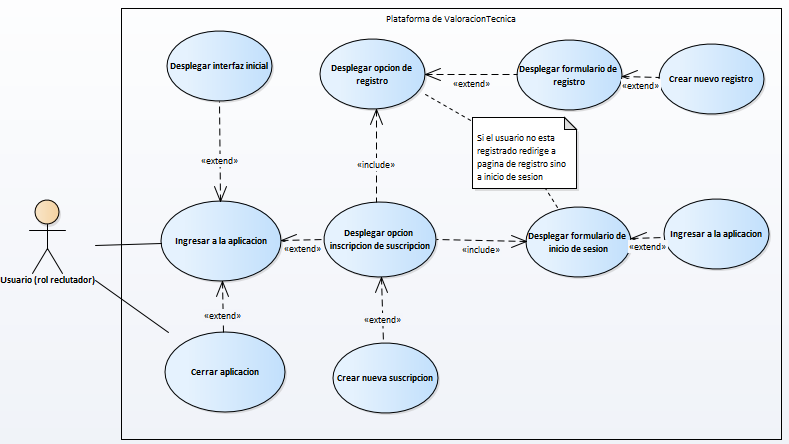
\includegraphics[width=0.9\textwidth]{Images/casoUso8.png}
    \fnote{Nota. \textup{Fuente : Autores.}}
    \end{minipage}
    

\newline
\textbf{Vistas principales del prototipo}
De acuerdo a los requerimientos funcionales y no funcionales junto con los casos de uso a continuación en las figuras \ref{prot1}, \ref{prot3}, \ref{prot4}, \ref{prot5} se adjuntan las vistas que representan el núcleo de nuestro plan de negocio. Todas las ilustraciones usadas en la creación de este prototipo fueron extraídas del sitio \textit{https://freesvgillustration.com} bajo la licencia de uso gratuito \cite{illustrations}.

    \vspace{2mm}
    \begin{minipage}{0.9\textwidth}
    \centering
    \captionof{figure}[{Vista principal}]{ Vista principal }
    \label{prot1}
     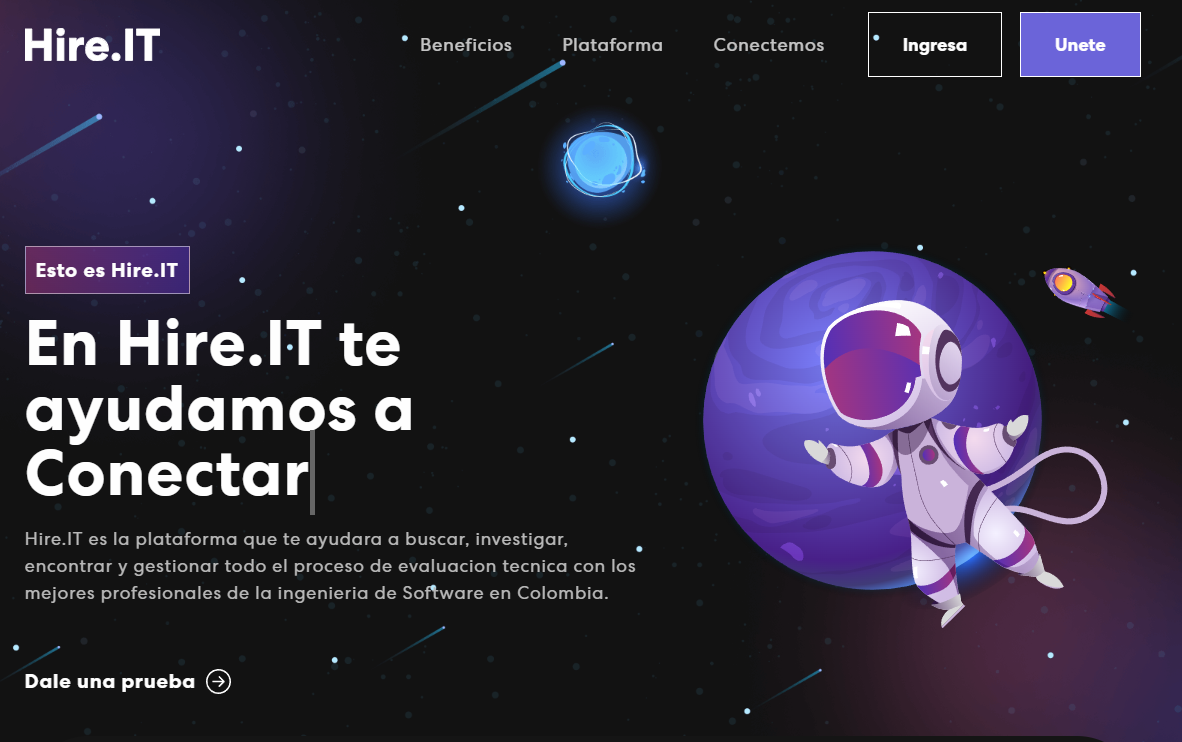
\includegraphics[width=0.7\textwidth]{Images/prot1.png}
    \fnote{Nota. \textup{Fuente: Autores}}
    \end{minipage}
    
    \vspace{2mm}
    \begin{minipage}{0.9\textwidth}
    \centering
    \captionof{figure}[{Vista registro}]{ Vista registro }
    \label{prot3}
     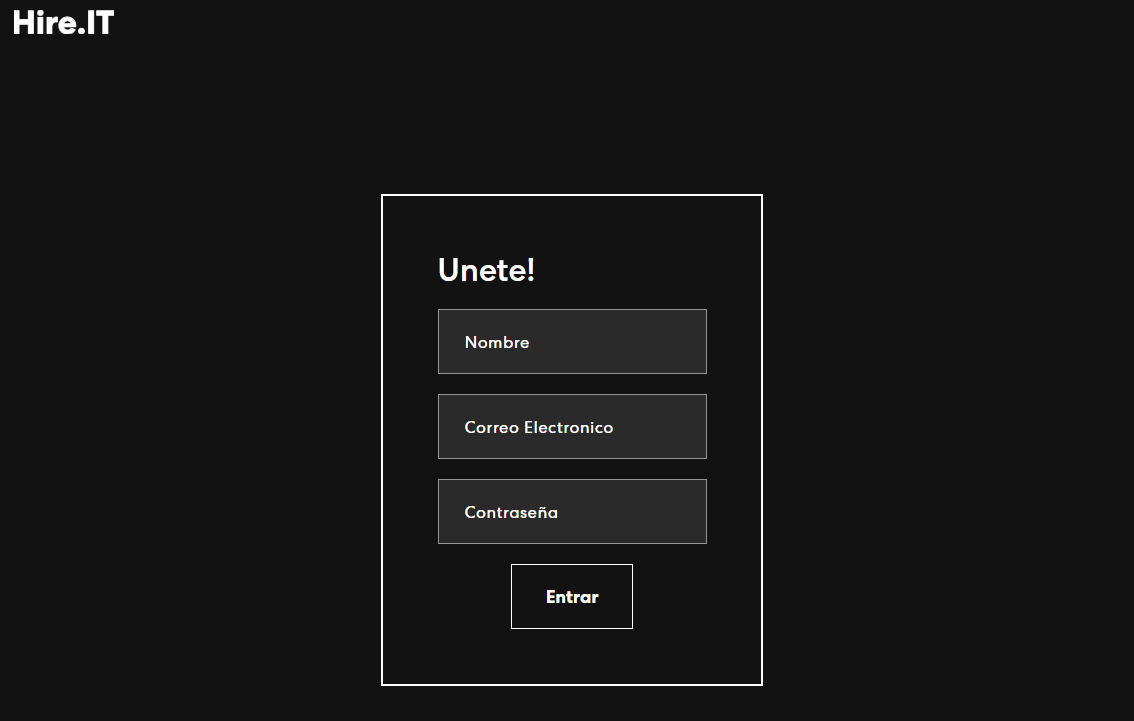
\includegraphics[width=0.7\textwidth]{Images/prot3.png}
    \fnote{Nota. \textup{Fuente: Autores}}
    \end{minipage}
    
    \vspace{2mm}
    \begin{minipage}{0.9\textwidth}
    \centering
    \captionof{figure}[{Vista marketing}]{ Vista marketing }
    \label{prot4}
     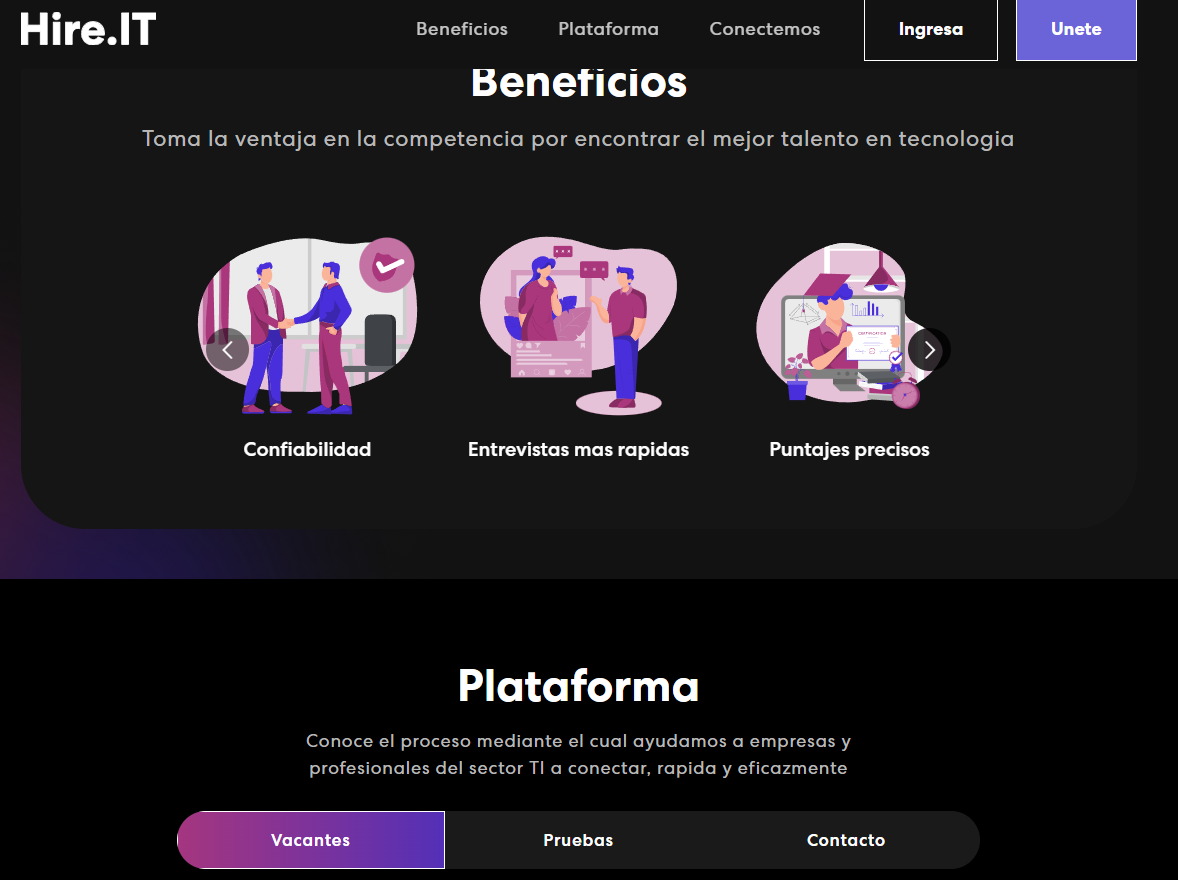
\includegraphics[width=0.7\textwidth]{Images/prot4.png}
    \fnote{Nota. \textup{Fuente: Autores}}
    \end{minipage}
    
    \vspace{2mm}
    \begin{minipage}{0.9\textwidth}
    \centering
    \captionof{figure}[{Vista contacto}]{ Vista contacto }
    \label{prot5}
     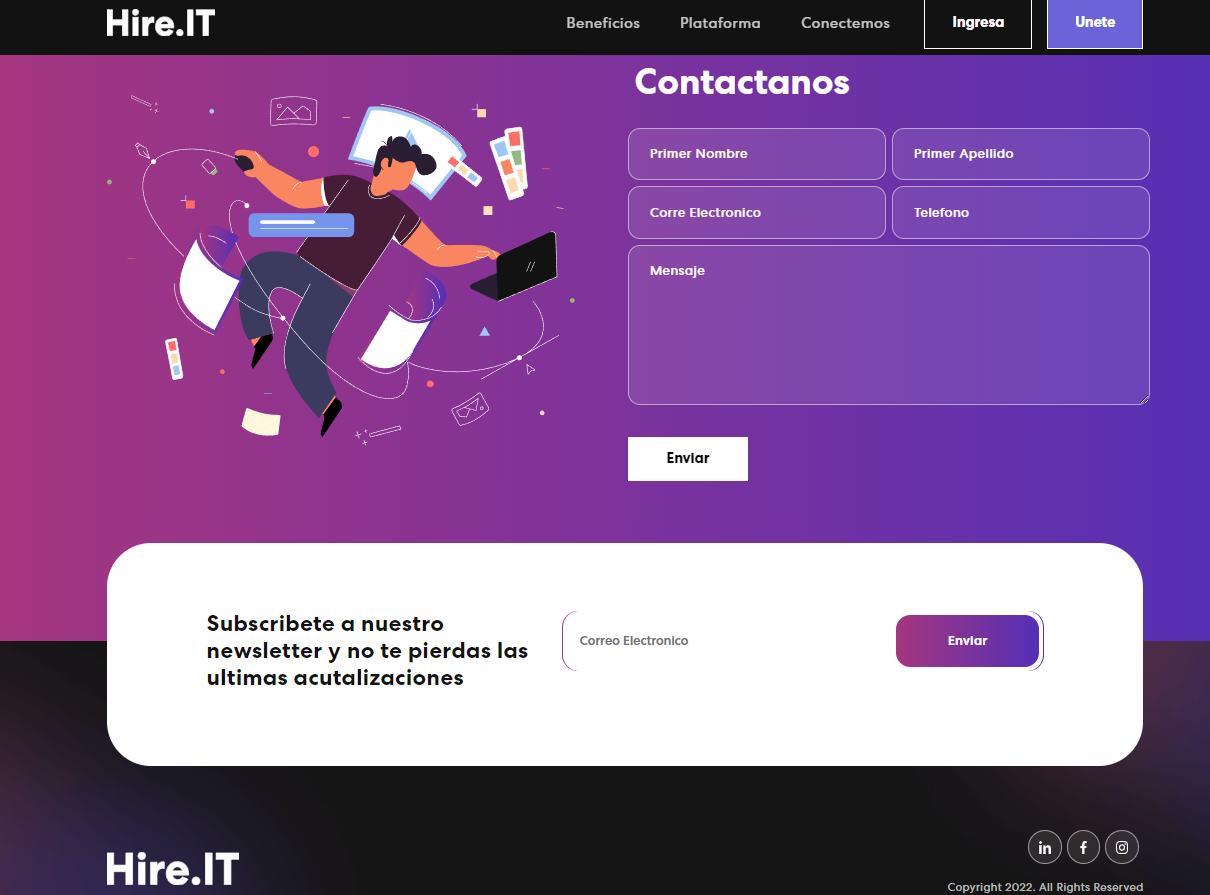
\includegraphics[width=0.7\textwidth]{Images/prot5.png}
    \fnote{Nota. \textup{Fuente: Autores}}
    \end{minipage}
    

